%
% $Id: wave.tex 1318 2007-09-26 04:39:14Z ksteube $
%
%%%%%%%%%%%%%%%%%%%%%%%%%%%%%%%%%%%%%%%%%%%%%%%%%%%%%%%
%
%           Copyright 2003-2007 by ACceSS MNRF
%       Copyright 2007 by University of Queensland
%
%                http://esscc.uq.edu.au
%        Primary Business: Queensland, Australia
%  Licensed under the Open Software License version 3.0
%     http://www.opensource.org/licenses/osl-3.0.php
%
%%%%%%%%%%%%%%%%%%%%%%%%%%%%%%%%%%%%%%%%%%%%%%%%%%%%%%%
%

\section{Rayleigh-Taylor Instability}
\label{LEVELSET CHAP}

In this chapter we will implement the Level Set Method in Escript for tracking the interface between two fluids for Computational Fluid Dynamics (CFD).
Normally in Earth science problems two or more fluids in a system with different properties are of interest. For example, lava dome growth in volcanology, with the contrast of the two mediums as being lava and air. The interface between the two mediums is often referred to as a free surface (free boundary value problem); the problem arises due to the large differences in densities between the lava and air, with their ratio being around 2000, and so the interface between the two fluids move with respect to each other.  
%and so the lava with the much higher density is able to move independently with respect to the air, and the interface between the two fluids is not constrained.
There are a number of numerical techniques to define and track the free surfaces. One of these methods, which is conceptually the simplest, is to construct a Lagrangian grid which moves with the fluid, and so it tracks the free surface. The limitation of this method is that it cannot track surfaces that break apart or intersect. Another limitation is that the elements in the grid can become severely distorted, resulting in numerical instability. The Arbitrary Lagrangian-Eulerian (ALE) method for CFD in moving domains is used to overcome this problem by remeshing, but there is an overhead in computational time, and it results in a loss of accuracy due to the process of mapping the state variables every remesh by interpolation.

There is a technique to overcome these limitations called the Level Set Method, for tracking interfaces between two fluids. The advantages of the method is that CFD can be performed on a fixed Cartesian mesh, and therefore problems with remeshing can be avoided. The field equations for calculating variables such as velocity and pressure are solved on the the same mesh. The Level Set Method is based upon the implicit representation of the interface by a continuous function. The function takes the form as a signed distance function, $\phi(x)$, of the interface in a Eulerian coordinate system. For example, the zero isocontour of the unit circle $\phi(x)=x^2 + y^2 -1$ is the set of all points where $\phi(x)=0$.
%
\begin{figure}
\center
\scalebox{0.5}{\includegraphics{figures/unitcircle.eps}}
\caption{Implicit representation of the curve $x^2 + y^2 = 1$.}
\label{UNITCIRCLE}
\end{figure}
%
The implicit representation can be used to define the interior and exterior of a fluid region. Since the isocontour at $\phi(x)=0$ has been defined as the interface, a point in the domain can be determined if its inside or outside of the interface, by looking at the local sign of $\phi(x)$. A point is inside the interface when $\phi(x)<0$, and outside the interface when $\phi(x)>0$. Parameters values such as density and viscosity can then be defined for two different mediums, depending on which side of the interface they are located. The displacement of the interface at the zero isocontour of $\phi(x)$ is calculated each time step by using the velocity field. This is achieved my solving the advection equation:

\begin{equation}
\frac{\partial \phi}{\partial t} + \vec{v} \cdot \nabla \phi = 0,
\label{ADVECTION}
\end{equation}

where $\vec{v}$ is the velocity field. The advection equation is solved using a mid-point method, which is a two step procedure:

Firstly, $\phi^{1/2}$ is calculated solving:

\begin{equation}
\frac{\phi^{1/2} - \phi^{-}}{dt/2} + \vec{v} \cdot \nabla \phi^{-} = 0.
\label{MIDPOINT FIST}
\end{equation}

Secondly, using $\phi^{1/2}$, $\phi^{+}$ is calculated solving:

\begin{equation}
\frac{\phi^{+} - \phi^{-}}{dt} + \vec{v} \cdot \nabla \phi^{1/2} = 0.
\label{MIDPOINT SECOND}
\end{equation}

For more details on the mid-point procedure see reference \cite{BOURGOUIN2006}. In certain situations the mid-point procedure has been shown to produce artifacts in the numerical solutions. A more robust procedure is to use the Taylor-Galerkin scheme with the presence of diffusion, which gives more stable solutions. The expression is derived by either inserting Equation (\ref{MIDPOINT FIST}) into Equation (\ref{MIDPOINT SECOND}), or by expanding $\phi$ into a Taylor series:

\begin{equation}
\phi^{+} \simeq \phi^{-} + dt\frac{\partial \phi^{-}}{\partial t} + \frac{dt^2}{2}\frac{\partial^{2}\phi^{-}}{\partial t^{2}},
\label{TAYLOR EXPANSION}
\end{equation}

by inserting

\begin{equation}
\frac{\partial \phi^{-}}{\partial t} = - \vec{v} \cdot \nabla \phi^{-},
\label{INSERT ADVECTION}
\end{equation}

and

\begin{equation}
\frac{\partial^{2} \phi^{-}}{\partial t^{2}} = \frac{\partial}{\partial t}(-\vec{v} \cdot \nabla \phi^{-}) = \vec{v}\cdot \nabla (\vec{v}\cdot \nabla \phi^{-}),
\label{SECOND ORDER}
\end{equation}

into Equation \ref{TAYLOR EXPANSION}

\begin{equation}
\phi^{+} = \phi^{-} - dt\vec{v}\cdot \nabla \phi^{-} + \frac{dt^2}{2}\vec{v}\cdot \nabla (\vec{v}\cdot \nabla \phi^{-}).
\label{TAYLOR GALERKIN}
\end{equation}
 

The fluid dynamics is governed by the Stokes equations. In geophysical problems the velocity of fluids are low; that is, the inertial forces are small compared with the viscous forces, therefore the inertial terms in the Navier-Stokes equations can be ignored. For a body force $f$ the governing equations are given by:

\begin{equation}
\nabla \cdot (\eta(\nabla \vec{v} + \nabla^{T} \vec{v})) - \nabla p = -f,
\label{GENERAL NAVIER STOKES}
\end{equation}

with the incompressibility condition

\begin{equation}
\nabla \cdot \vec{v} = 0.
\label{INCOMPRESSIBILITY}
\end{equation}

where $p$, $\eta$ and $f$ are the pressure, viscosity and body forces, respectively. 
Alternatively, the Stokes equations can be represented in Einstein summation tensor notation (compact notation):

\begin{equation}
-(\eta(v\hackscore{i,j} + v\hackscore{j,i})),\hackscore{j} - p,\hackscore{i} = f\hackscore{i},
\label{GENERAL NAVIER STOKES COM}
\end{equation}

with the incompressibility condition

\begin{equation}
-v\hackscore{i,i} = 0.
\label{INCOMPRESSIBILITY COM}
\end{equation}

The subscript $,i$ denotes the derivative of the function with respect to $x\hackscore{i}$. A linear relationship between the deviatoric stress $\sigma^{'}\hackscore{ij}$ and the stretching $D\hackscore{ij} = \frac{1}{2}(v\hackscore{i,j} + v\hackscore{j,i})$ is defined as \cite{GROSS2006}:

\begin{equation}
\sigma^{'}\hackscore{ij} = 2\eta D^{'}\hackscore{ij},
\label{STRESS}
\end{equation}

where the deviatoric stretching $D^{'}\hackscore{ij}$ is defined as

\begin{equation}
D^{'}\hackscore{ij} = D^{'}\hackscore{ij} - \frac{1}{3}D\hackscore{kk}\delta\hackscore{ij}.
\label{DEVIATORIC STRETCHING}
\end{equation}

The $\delta\hackscore{ij}$ is the Kronecker $\delta$-symbol, which is a matrix with ones for its diagonal entries ($i = j$) and zeros for the remaining entries ($i \neq j$). The body force $f$ in Equation (\ref{GENERAL NAVIER STOKES COM}) is the gravity acting in the $x\hackscore{3}$ direction and is given as $f = -g \rho \delta\hackscore{i3}$.

The Stokes equations is a saddle point problem, and can be solved using a Uzawa scheme. A class called StokesProblemCartesian in Escript can be used to solve for velocity and pressure.
In order to keep numerical stability, the time step size needs to be below a certain value, known as the Courant number. The Courant number is defined as:

\begin{equation}
C = \frac{v \delta t}{h}.
\label{COURANT}
\end{equation}

where $\delta t$, $v$, and $h$ are the time step, velocity, and the width of an element in the mesh, respectively. The velocity $v$ may be chosen as the maximum velocity in the domain. In this problem the Courant number is taken to be 0.4 \cite{BOURGOUIN2006}.

As the computation of the distance function progresses, it becomes distorted, and so it needs to be updated in order to stay regular. This process is known as the reinitialization procedure. The aim is to iteratively find a solution to the reinitialization equation:

\begin{equation}
\frac{\partial \psi}{\partial \tau} + sign(\psi)(1 - \nabla \psi) = 0.
\label{REINITIALISATION}
\end{equation}

where $\tau$ is artificial time. This equation is solved to meet the definition of the level set function, $\lvert \nabla \psi \rvert = 1$; the normalization condition. However, it has been shown that in using this reinitialization procedure it is prone to mass loss and inconsistent positioning of the interface \cite{SUCKALE2008}.

The Rayleigh-Taylor instability problem is used as a benchmark to validate CFD implementations \cite{VANKEKEN1997}. Figure \ref{RT2DSETUP} shows the setup of the problem. A rectangular domain with two different fluids is considered, with the greater density fluid on the top and the lighter density fluid on the bottom. The viscosities of the two fluids are equal (isoviscos). An initial perturbation is given to the interface of $\phi=0.02cos(\frac{\pi x}{\lambda}) + 0.2$. The aspect ratio, $\lambda = L/H = 0.9142$, is chosen such that it gives the greatest disturbance of the fluids.

\begin{figure}
\center
\scalebox{0.7}{\includegraphics{figures/RT2Dsetup.eps}}
\caption{Parameters, initial interface and boundary conditions for the Rayleigh-Taylor instability problem. The interface is defined as $\phi=0.02cos(\frac{\pi x}{\lambda}) + 0.2$. The fluids have been assigned different densities and equal viscosity (isovisous).}
\label{RT2DSETUP}
\end{figure}

%The Level Set Method can be applied to many areas of science, for example simulating subduction zones in geophysics, motion of bubbles, and flame propagation. Its also used in image processing. However, the Level Set Method does have limitations. The level set function can still become irregular after reinitialisation, leading to artifacts in the simulations, requiring more thought into the implementation of the reinitialisation step.
